\section{Giải thuật}
\subsection{Giải thuật đề xuất bài học}
Khi người dùng cung cấp mục tiêu học tập, hệ thống sử dụng LLM để phân tích và xác định các khái niệm quan trọng. Các khái niệm này được trích xuất từ mục tiêu học tập thông qua LLM, và được lưu trữ trong cơ sở dữ liêu đồ thị (graph database) Neo4j. Neo4j sẽ là cơ sở dữ liệu đồ thị để lưu trữ và quản lý các khái niệm học tập, tài nguyên học tập, và mối quan hệ giữa chúng. Đồ thị này bao gồm hai loại thực thể chính: \textbf{Node} (điểm nút) và \textbf{Relationship} (mối quan hệ). Dưới đây là chi tiết về cấu trúc đồ thị:

Các loại node trong hệ thống bao gồm:
\begin{itemize}
    \item \textbf{Concept:}  Mỗi node sẽ đại diện cho một khái niệm học tập.
    \item \textbf{Learning Resource:} Các node tài nguyên học tập sẽ đại diện cho các bài giảng, sách, video, tài liệu học tập, ví dụ: "Video bài giảng về phương trình bậc hai", "Bài viết về đạo hàm".
    \item \textbf{Learner:} Node người học sẽ chứa thông tin về người học, bao gồm các khái niệm mà họ đang học và mức độ thành thạo của họ đối với từng khái niệm.
\end{itemize}
Các mối quan hệ giữa các node sẽ bao gồm:
\begin{itemize}
    \item \textbf{COVERS:} Quan hệ giữa tài nguyên học tập và khái niệm mà tài nguyên đó đề cập đến. Ví dụ: Một video có thể "COVERS" khái niệm "Phương trình bậc hai". Mối quan hệ này sẽ có một thuộc tính difficulty (độ khó).
    \item \textbf{LEARNS:}  Quan hệ giữa người học và khái niệm mà họ đang học. Ví dụ: Người học "LEARNS" khái niệm "Lập trình Python". Mối quan hệ này sẽ có một thuộc tính proficiency (độ thành thạo) để xác định người học đã nắm vững khái niệm đó đến mức nào.
\end{itemize}
Để trích xuất các khái niệm liên quan, hệ thống sử dụng kỹ thuật vector embedding để chuyển đổi khái niệm và tài nguyên học tập thành các vector đại diện. Mỗi khái niệm và tài nguyên học tập sẽ có một vector tương ứng trong không gian nhiều chiều.
\begin{itemize}
    \item \textbf{Vector Embedding:}  Mỗi khái niệm và tài nguyên học tập được chuyển thành một vector nhờ các phương pháp như Word2Vec, BERT hoặc các mô hình ngôn ngữ khác. Các vector này giúp biểu diễn sự tương đồng ngữ nghĩa giữa các khái niệm và tài nguyên.
    \item \textbf{Cosine Similarity:} Sau khi có vector cho mỗi khái niệm và tài nguyên học tập, hệ thống sử dụng cosine similarity để tính toán sự tương đồng giữa các khái niệm mà người học cần thành thạo và các tài nguyên học tập có sẵn. Cosine similarity được tính bằng công thức:
$$
\text{Cosine Similarity} = \frac{\mathbf{A} \cdot \mathbf{B}}{\|\mathbf{A}\| \cdot \|\mathbf{B}\|}
$$

\end{itemize}
\subsection{Workflow của LLM và Function Calling}
LLM đóng vai trò quan trọng trong việc trích xuất các khái niệm và giải thích tài nguyên học tập. LLM sẽ thực hiện các tác vụ sau:
\subsubsection{Phân tích Mục tiêu và Xác định Khái niệm
}
Khi nhận được mục tiêu học tập từ người dùng, LLM sẽ phân tích mục tiêu này và xác định các khái niệm cần thiết. Ví dụ, nếu mục tiêu học tập là "Làm chủ lập trình Python", LLM có thể trích xuất các khái niệm như "Biến", "Câu lệnh điều kiện", "Vòng lặp",...
\subsubsection{Function Calling để Trích xuất Dữ liệu
}
Sau khi LLM xác định các khái niệm, LLM sẽ sử dụng function calling để gọi các hàm trong hệ thống nhằm trích xuất các thông tin sau:
\begin{itemize}
    \item Thông tin người học: LLM gọi hàm để lấy các khái niệm mà người học đã học, cùng với mức độ thành thạo đối với các khái niệm này.
    \item Thông tin tài nguyên học tập: LLM gọi hàm để lấy danh sách các tài nguyên học tập có sẵn, bao gồm các tài nguyên đã được gán các khái niệm và độ khó của chúng.
\end{itemize}
\subsubsection{Trích xuất và Đề xuất Tài nguyên Học tập
}
LLM sẽ sử dụng thông tin về người học và tài nguyên học tập để tính toán độ phù hợp giữa người học và tài nguyên học tập. Cụ thể:
\begin{itemize}
    \item Dựa vào cosine similarity giữa các vector của khái niệm và tài nguyên học tập.
    \item Xác định những tài nguyên học tập phù hợp nhất cho người học dựa trên mức độ thành thạo của họ và độ khó của tài nguyên học tập.

\end{itemize}
\subsubsection{ Giải thích kết quả}
Sau khi đã chọn ra các tài nguyên học tập, LLM sẽ tiếp tục sử dụng function calling để tạo ra giải thích chi tiết về cách mỗi tài nguyên giúp người học cải thiện khả năng thành thạo các khái niệm cần thiết. LLM sẽ trả về các giải thích dạng tự nhiên cho người học.
\begin{figure}[H]
    \centering
    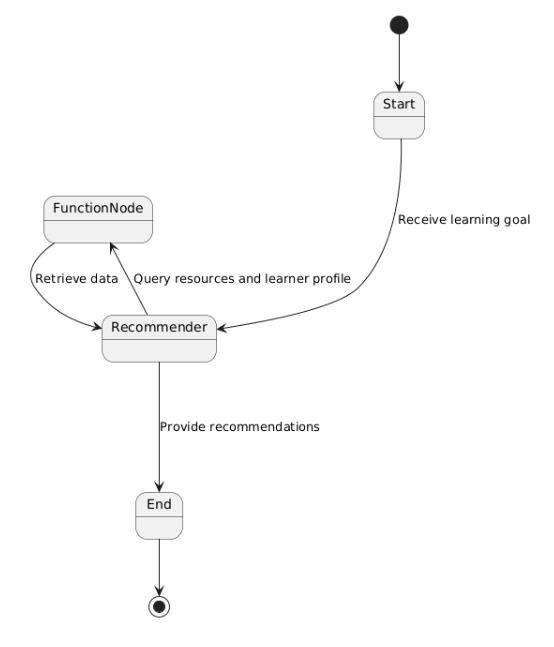
\includegraphics[width=0.7\linewidth]{Images/Anh/giaithuat.png}
    \caption{Flowchart giải thuật đề xuất bài học}
    \label{fig:enter-label}
\end{figure}